\documentclass[a4paper,papersize,dvipdfmx]{jsarticle}
\usepackage{ascmac}
\usepackage{mathtools, amssymb,bm}
\usepackage{comment}
\usepackage[hiresbb]{graphicx}
\usepackage{tcolorbox,color}
\usepackage{here}
\tcbuselibrary{raster,skins,breakable}

\newcommand{\pic}[1]{\begin{center} \includegraphics[width=1.0\linewidth,clip]{#1} \end{center}}   %写真用
\newcommand{\pict}[2]{\begin{center} \includegraphics[width= {#2} cm]{#1} \end{center}}   %写真用
\newcommand{\redunderline}[1]{\textcolor{red}{\underline{¥textcolor{black}{#1}}}}   %赤いアンダーライン
\newcommand{\mon}[1]{\item[({#1})] \ }
\newcommand{\ctext}[1]{\raise0.2ex\hbox{\textcircled{\scriptsize{#1}}}}%文字を丸囲みする(2桁の数字までならいける)

% 画像を貼る時はjpgかjpegで、pngはうまくいかないっぽい

%\itemを四角で囲った数字にする場合は以下のコメントアウトを消す
%\renewcommand{\labelenumi}{\textbf{\framebox[1.5zw]{\theenumi}}}


%enumerateの2階層めのカウンタを1,2,3, にする時は以下のコメントアウトを消す
\renewcommand{\theenumii}{\arabic{enumii}}

%enumerateのカウンタについては以下を参照
% http://www3.otani.ac.jp/fkdsemi/pLaTeX_manual/kajyo.html


%enumerateの番号の出力形式を変更するには、カウンタの値を出力する命令を定義し直す。
%レベル	カウンタ	出力する命令	デフォルトの出力
%1	enumi	¥theenumi	アラビア数字(1,2,3,・・・)
%2	enumii	¥theenumii	小文字のアルファベット(a,b,c,・・・)
%3	enumiii	¥theenumiii	小文字のローマ数字(小文字のローマ数字(\UTF{2170},\UTF{2171},\UTF{2172},・・・)
%4	enumiv	¥theenumiv	大文字のアルファベット(A,B,C,・・・)
%例:¥enumiカウンタを大文字のローマ数字で出力する設定
% ¥renewcommand{¥theenumi}{¥Roman{enumi}}

% 番号の出力形式
%命令	出力形式
%¥arabic	アラビア数字(1、2、3、・・・)
%¥roman	ローマ数字(\UTF{2170}、\UTF{2171}、\UTF{2172}、・・・)
%¥Roman	ローマ数字(\UTF{2160}、\UTF{2161}、\UTF{2162}、・・・)
%¥alph	アルファベット(a、b、c、・・・)
%¥Alph	アルファベット(A、B、C、・・・)




\begin{document}

\title{蛋白構造生物学教室}
\author{10191043 鈴木健一}
%作成日を入れる場合は消す
\date{}
\maketitle

%以下の3つからフォントサイズを選択するとよい
%\footnotesize
%\small
%\normalsize


\begin{flushright}
実験日 : 2019/6/25 $\sim$ 2019/6/28

共同実験者 : 須藤成俊
\end{flushright}

\part*{1日目}

\section*{実験操作}
\subsection*{ニワトリ卵白溶液の調製}
次のイオン交換樹脂で精製するための卵白溶液を調製する。

\subsection*{イオン交換樹脂を用いた精製}
イオン交換樹脂を用いてニワトリ卵白リゾチームを溶出し、吸光度の測定によって最もリゾチーム濃度の濃い分画をとる。

\subsection*{ニワトリ卵白リゾチームの結晶化用溶液作成}
前項でとったリゾチーム分画を遠心による限外濾過で濃縮する。

\section*{結果および課題}

\begin{tcolorbox}[colback=white,colbacktitle=black,coltitle=white,title={1.}]
リゾチームのアミノ酸配列からモル吸光係数を計算し、溶出分画のリゾチーム濃度を計算する。
\end{tcolorbox}

実習書3-3より、リゾチーム1配列あたりにトリプトファンは6残基、チロシンは3残基含まれることからモル吸光係数は以下のようになる。

\[\epsilon_{280}^{1cm}=5690 \times6+1280 \times 3 = 37980\]

また、1から3分画までの吸光度を測定した結果、以下のようになった。
タンパク質濃度はLambert-Beerの法則を用いて希釈率と吸光度から算出した。

\begin{table}[H]
\begin{center}
\begin{tabular}{|c|c|c|c|}
\hline
画分  & 1     & 2     & 3     \\ \hline
希釈率  & 1/50     & 1/10     & 1/2     \\ \hline
吸光度 & 0.168 & 0.159 & 0.345 \\ \hline
タンパク質濃度 & $2.21 \cdot 10^{-4}$& $4.19 \cdot 10^{-5}$&$1.81 \cdot 10^{-5}$ \\ \hline
\end{tabular}
\end{center}
\end{table}

したがって最も濃い分画の濃度は $2.21 \cdot 10^{-4}$ mol/Lである。ゾチームの分子量が14.3 kDaなので、求めるリゾチーム濃度は3.16 mg/mL となる。

\begin{tcolorbox}[colback=white,colbacktitle=black,coltitle=white,title={2.}]
ニワトリ蛋白半分からリゾチームが何mg精製できたかを計算する。
\end{tcolorbox}

1番目の溶出分画は約7.0 mLだったので、精製できたリゾチームは22.1 mgである。

\part*{2日目}

\section*{実験操作}

\subsection*{リゾチームの結晶化用溶液作成}

30$\sim$50 mg/ml程度になるまで限外濾過で濃縮する。


\subsection*{SDS-PAGEによる精製の確認}

SDS-PAGEによって卵白溶液、陽イオン交換樹脂に結合しなかった画分、洗浄画分、溶出画分の組成を確認する。


\subsection*{ニワトリ卵白リゾチームの結晶化}
蒸気拡散法によるリゾチーム結晶化の準備をする。塩化ナトリウム0.6 M、1.0 M、1.4 M、pH 4.7の条件で卵白から精製したリゾチーム溶液と市販のリゾチーム溶液を結晶化させた。

\section*{結果および課題}
\begin{tcolorbox}[colback=white,colbacktitle=black,coltitle=white,title={(1)}]
分子量マーカーバンドの泳動度から検量線を作成し、リゾチームのバンドを見つけ、精製が成功しているかを判断する。
\end{tcolorbox}

SDS-PAGEを結果、以下のようにゲルが染色された。

\pict{imgs/row-gel.jpg}{4}

分子量マーカー、およびそれと泳動度の関係をプロットし、それに沿うような検量線を対数近似と累乗近似の2通りで引いた。

\subsubsection*{対数近似}
\pict{imgs/gel.png}{8}

検量線を引いた結果、以下のような式が得られた。

\[\rm{Migration \ degree} = -1.622 \times \ln(\rm{Molecular \ weight}) + 9.053\]

決定係数は0.9534であり、濃度が小さい領域で合致しているが、任意の分子量で泳動度が得られた近似式にフィットすると考えると、濃度が十分に大きい領域では泳動度が負になってしまうので近似曲線としては適していないように思われる。

\subsubsection*{累乗近似}
\pict{imgs/gel-2.png}{8}

検量線を引いた結果、以下のような式が得られた。

\[\rm{Migration \ degree} = 23.91 \times \rm{Molecular \ weight}^{-0.5973}\]

決定係数は0.9809と対数近似よりもプロットした値にフィットしている。こちらのモデルの方が泳動度の近似曲線として適していると考えられる。


また、他の泳動レーンに現れたバンドは以下のようになった。

\begin{table}[H]
\begin{center}
\begin{tabular}{|c|c|c|c|c|c|c|c|c|}
\hline
泳動度(cm)            & 1   & 2   & 3   & 4   & 5   & 6   & 7   & 8   \\ \hline
卵白溶液               & 0.5 & 0.8 & 1.7 & 2.6 & 3.5 & 4.1 & 4.7 & 5.2 \\ \hline
陽イオン交換樹脂に結合しなかった画分 & 0.5 & 0.8 & 1.7 & 2.6 & 3.5 & 4.1 & 4.7 & 5.2 \\ \hline
3回目の溶出区分           & 5.2 &     &     &     &     &     &     &     \\ \hline
溶出区分               & 5.2 &     &     &     &     &     &     &     \\ \hline
市販のリゾチーム溶液         & 5.2 & 5.5 & 5.6 & 5.8 &     &     &     &     \\ \hline
\end{tabular}
\end{center}
\end{table}

溶出画分からは5.2cmのバンドのみが得られた。累乗近似の曲線の方程式に泳動度5.2 cmを代入すると、12.86 kDaとなり、リゾチームの分子量14.3 kDaに近いので、これがリゾチームのバンドであると思われる。


\begin{tcolorbox}[colback=white,colbacktitle=black,coltitle=white,title={(2)}]
結晶化に用いる精製試料中にはリゾチームのみが含まれているのが理想的である。今回の精製操作では夾雑物を含む可能性がある。なぜか考察せよ。さらに精製純度を上げるためにはどのような操作を行えば良いか考察する。
\end{tcolorbox}

実習書にはリゾチームと等電点が近く、分子量が68.3のAvidinがニワトリ卵白中のタンパク質に含まれていると記載されている。イオン交換クロマトグラフィーにおいてリゾチームと等電点が近いAvidinも溶出し夾雑物として染色バンドが現れることが考えられる。
そこでリゾチームの純度さらにを上げるためには、pHを調整したイオン交換クロマトグラフィーを繰り返し行って夾雑物を排除することや、分子ふるい効果によって分子量の異なる者を排除するクロマトグラフィーも行うことが考えられる。

\part*{3日目}
\section*{実験操作}

\subsection*{ニワトリ卵白リゾチームの結晶の観察}
結晶化したリゾチームを実体顕微鏡で観察する。

\subsection*{ニワトリ卵白リゾチームのX線回折実験}
X線回折計を用いてリゾチームの結晶の回折像を得る。

\section*{結果および課題}

\begin{tcolorbox}[colback=white,colbacktitle=black,coltitle=white,title={1}]
結晶のでき方は、数個の大きくて形のはっきりしたものができる場合と、小さなものがシャワー状になってできる場合、あるいは全くできない場合がある。今回の6種類の結晶化条件では、どのような結果が期待できるか。理由とともに述べよ。また実際の結果を記載せよ。
\end{tcolorbox}

それぞれの条件で結晶を観察した結果は以下のようになった。

\begin{table}[H]
\begin{center}
\begin{tabular}{|c|c|c|c|c|}
\hline
リゾチーム & リザーバー条件 & 結晶の数 & 大きさ(μm) & 外形   \\ \hline
市販    & 1       & 35   & 270     & 正六角柱 \\ \hline
市販    & 2       & 8    & 111     & 正六角柱 \\ \hline
市販    & 3       & 0    & -       & -    \\ \hline
精製    & 1       & 1    & 325     & 正六角柱 \\ \hline
精製    & 2       & 0    & -       & -    \\ \hline
精製    & 3       & 0    & -       & -    \\ \hline
\end{tabular}
\end{center}
\end{table}

また結晶が見られたものについては以下に画像を添付している。倍率は40倍である。

\begin{figure}[H]
\begin{center}
\begin{tabular}{c}

\begin{minipage}{0.22\hsize}
\begin{center}
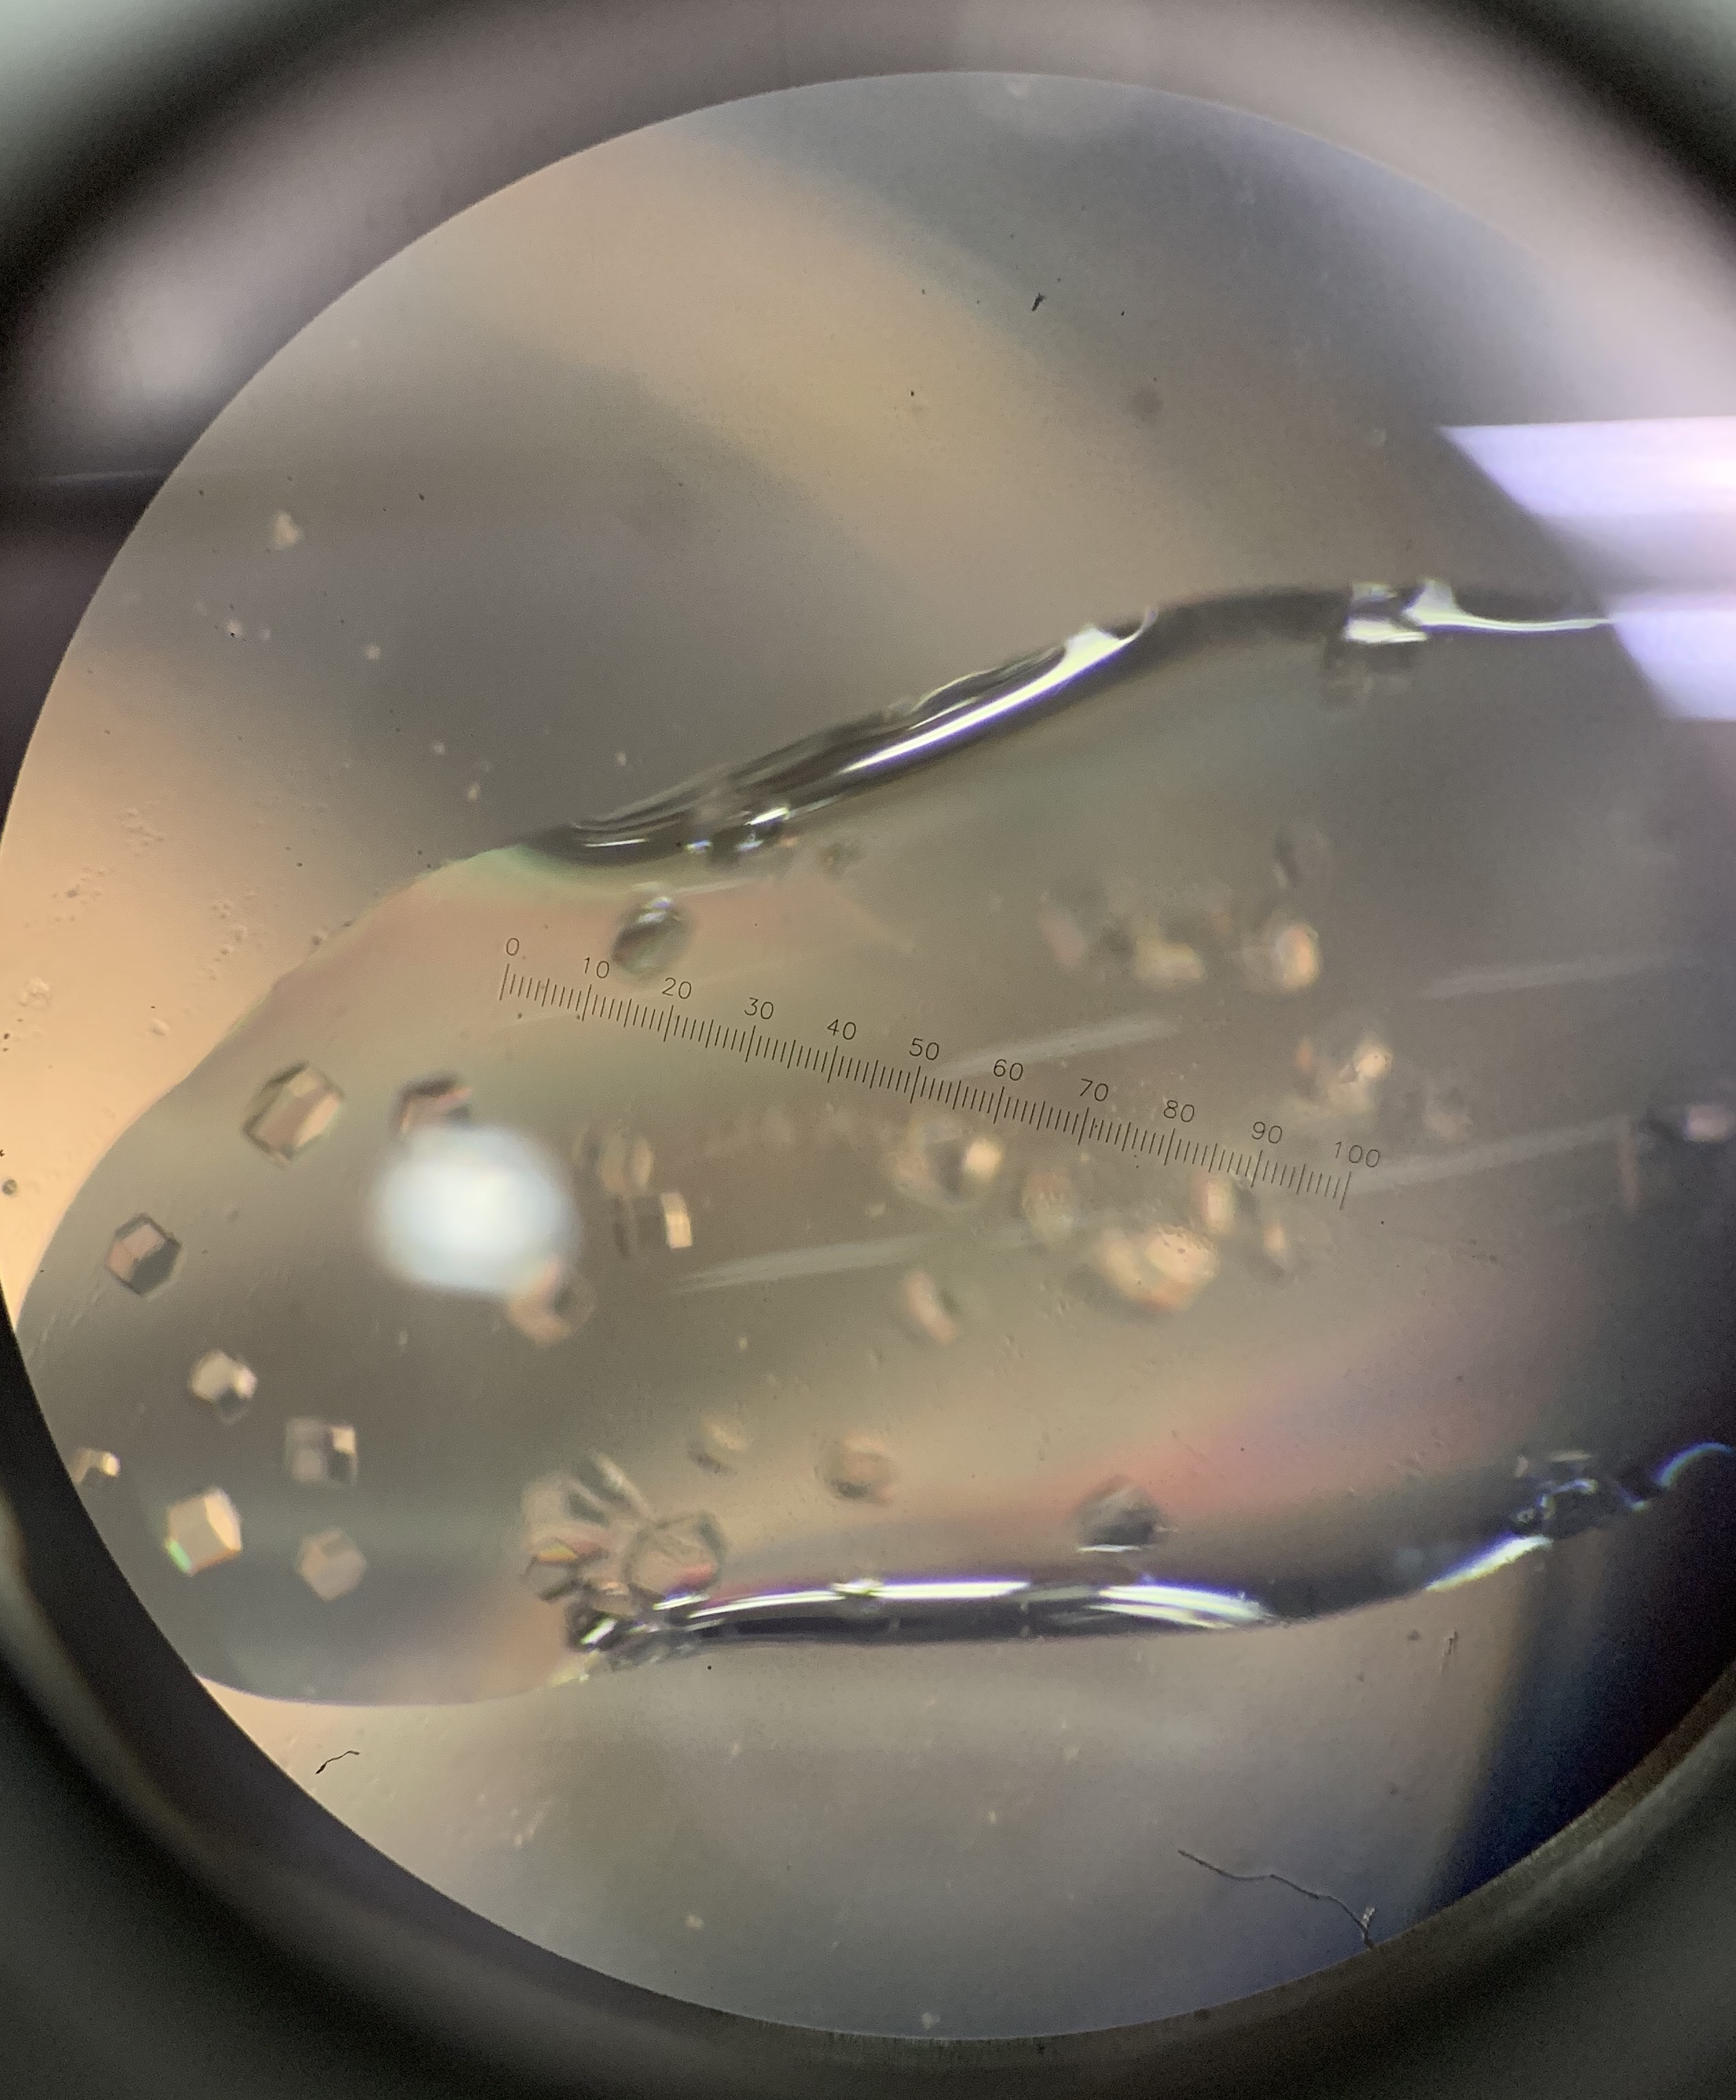
\includegraphics[clip, height=4cm]{imgs/s-1.jpg}
\hspace{1.6cm} 市販-1
\end{center}
\end{minipage}

\begin{minipage}{0.05\hsize}
\hspace{2mm}
\end{minipage}

\begin{minipage}{0.22\hsize}
\begin{center}
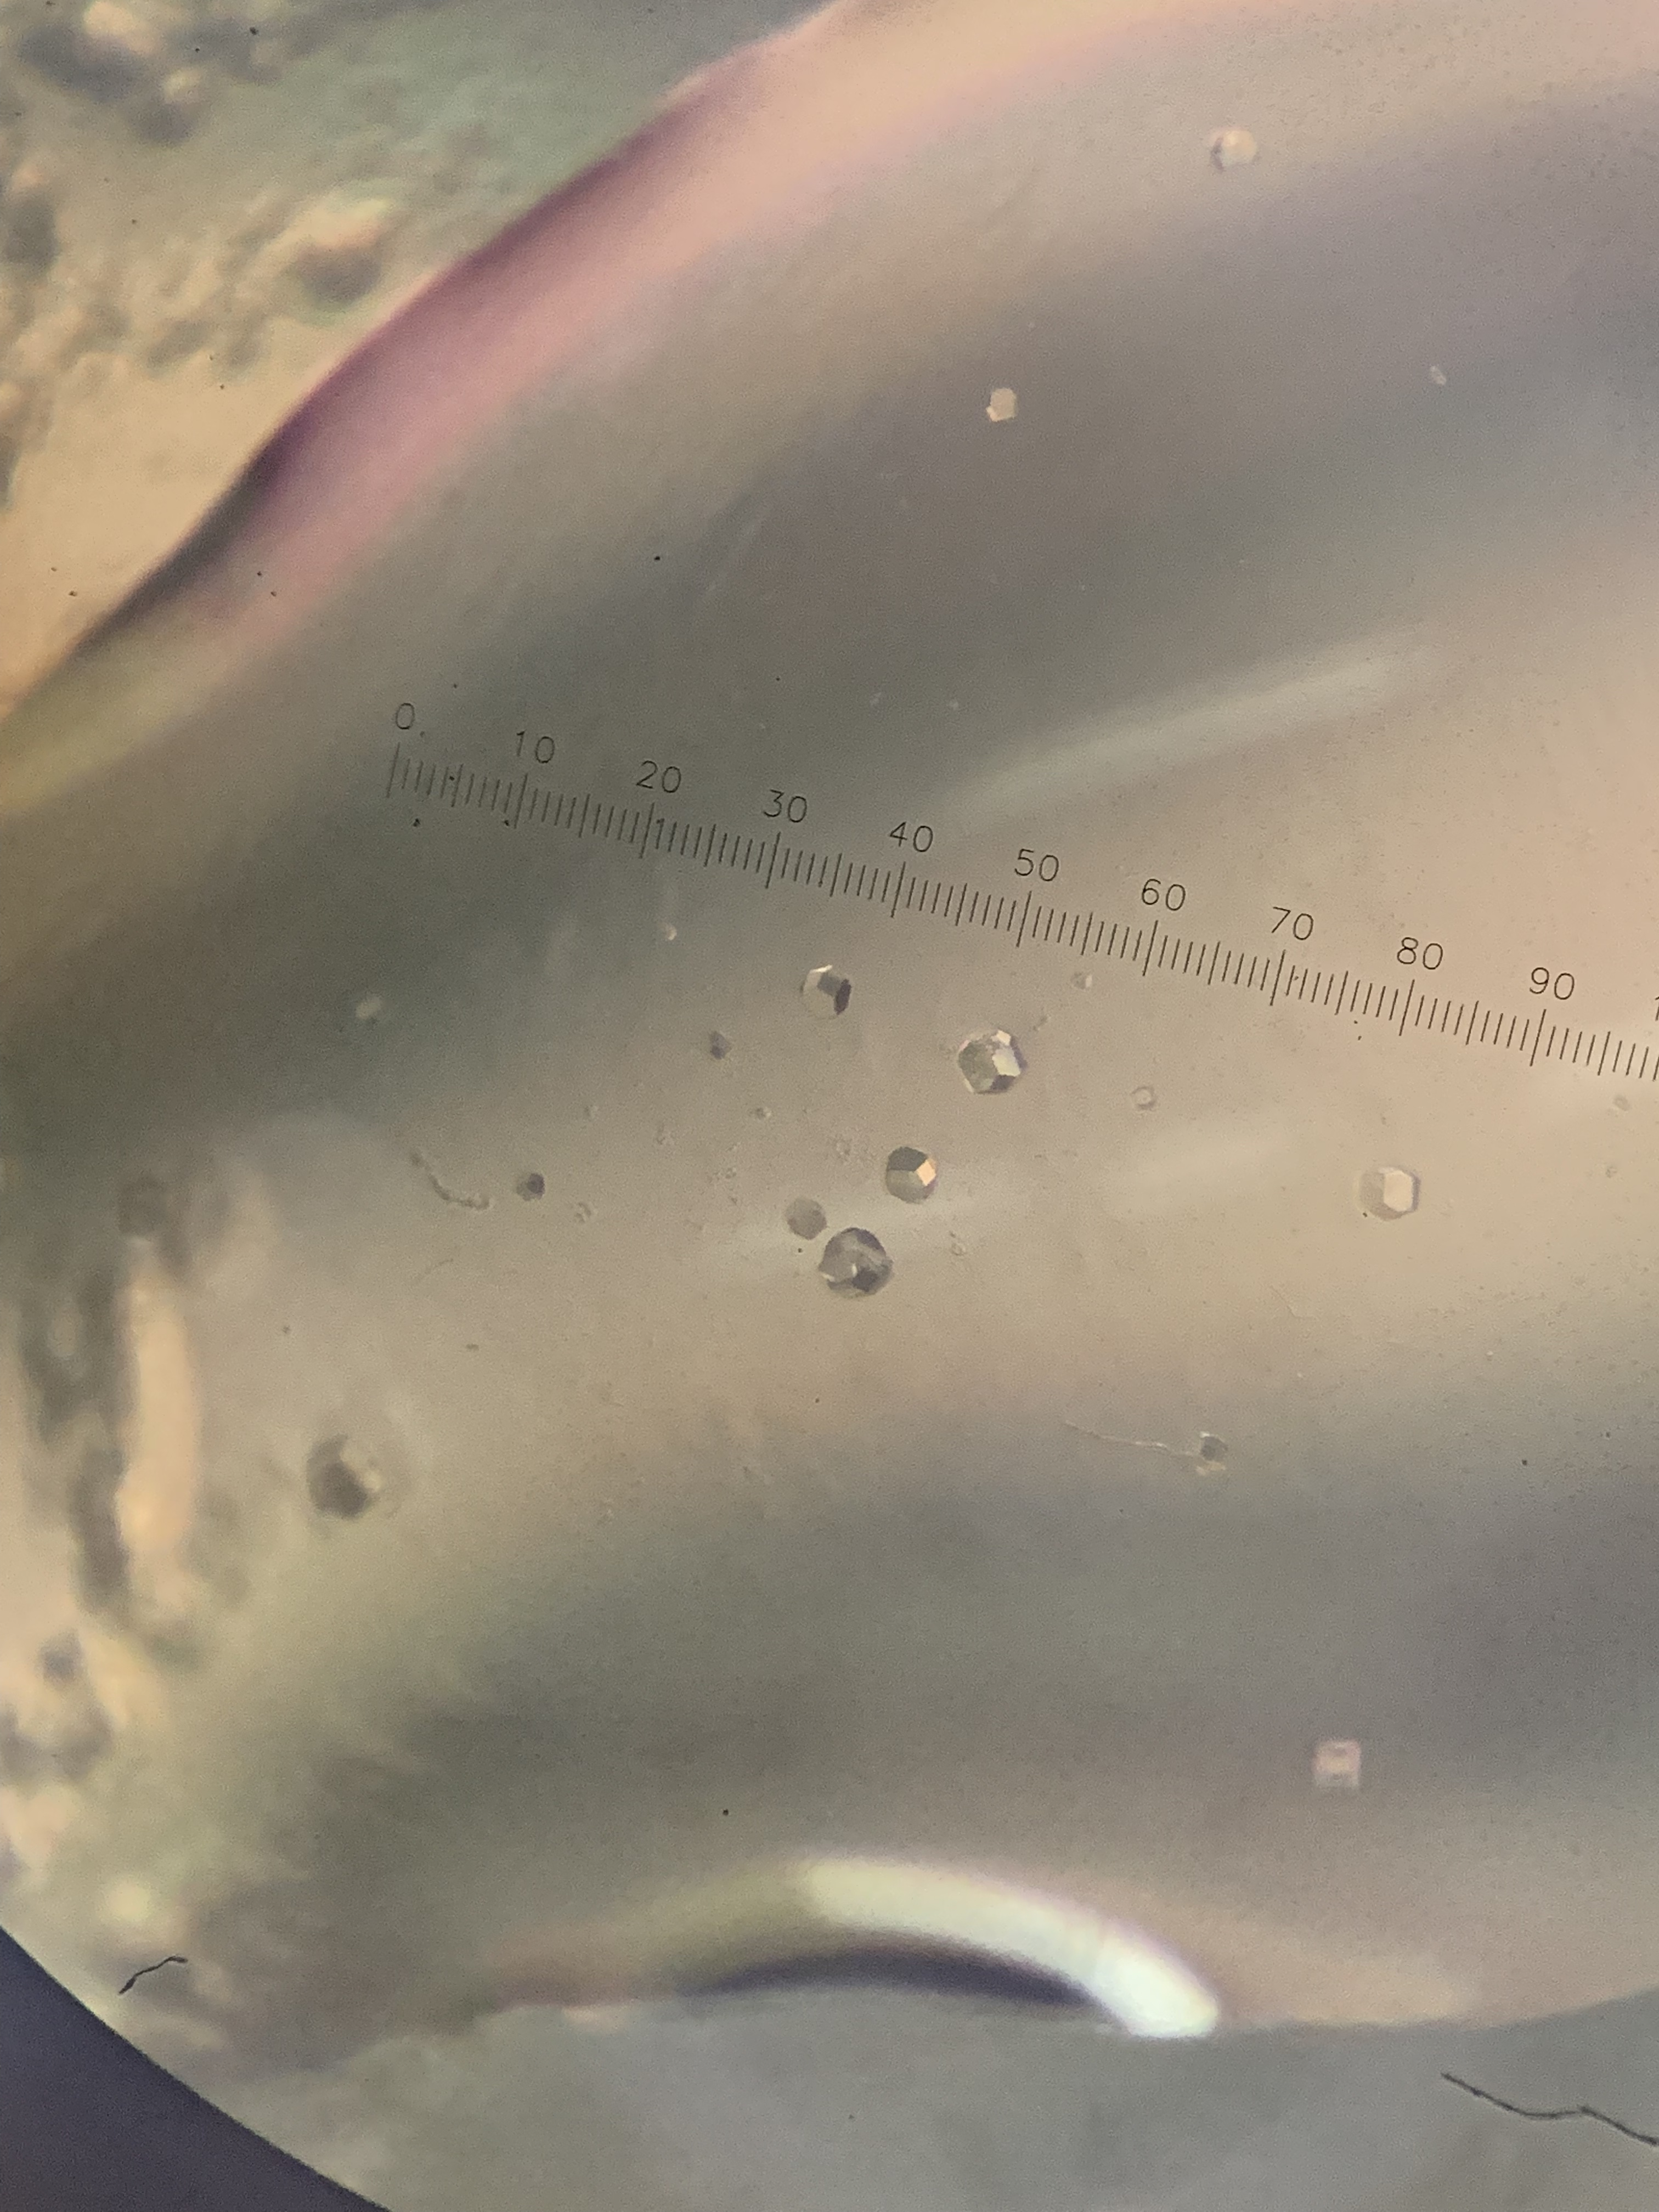
\includegraphics[clip, height=4cm]{imgs/s-2.jpg}
\hspace{1.6cm} 市販-2
\end{center}
\end{minipage}

\begin{minipage}{0.05\hsize}
\hspace{2mm}
\end{minipage}

\begin{minipage}{0.22\hsize}
\begin{center}
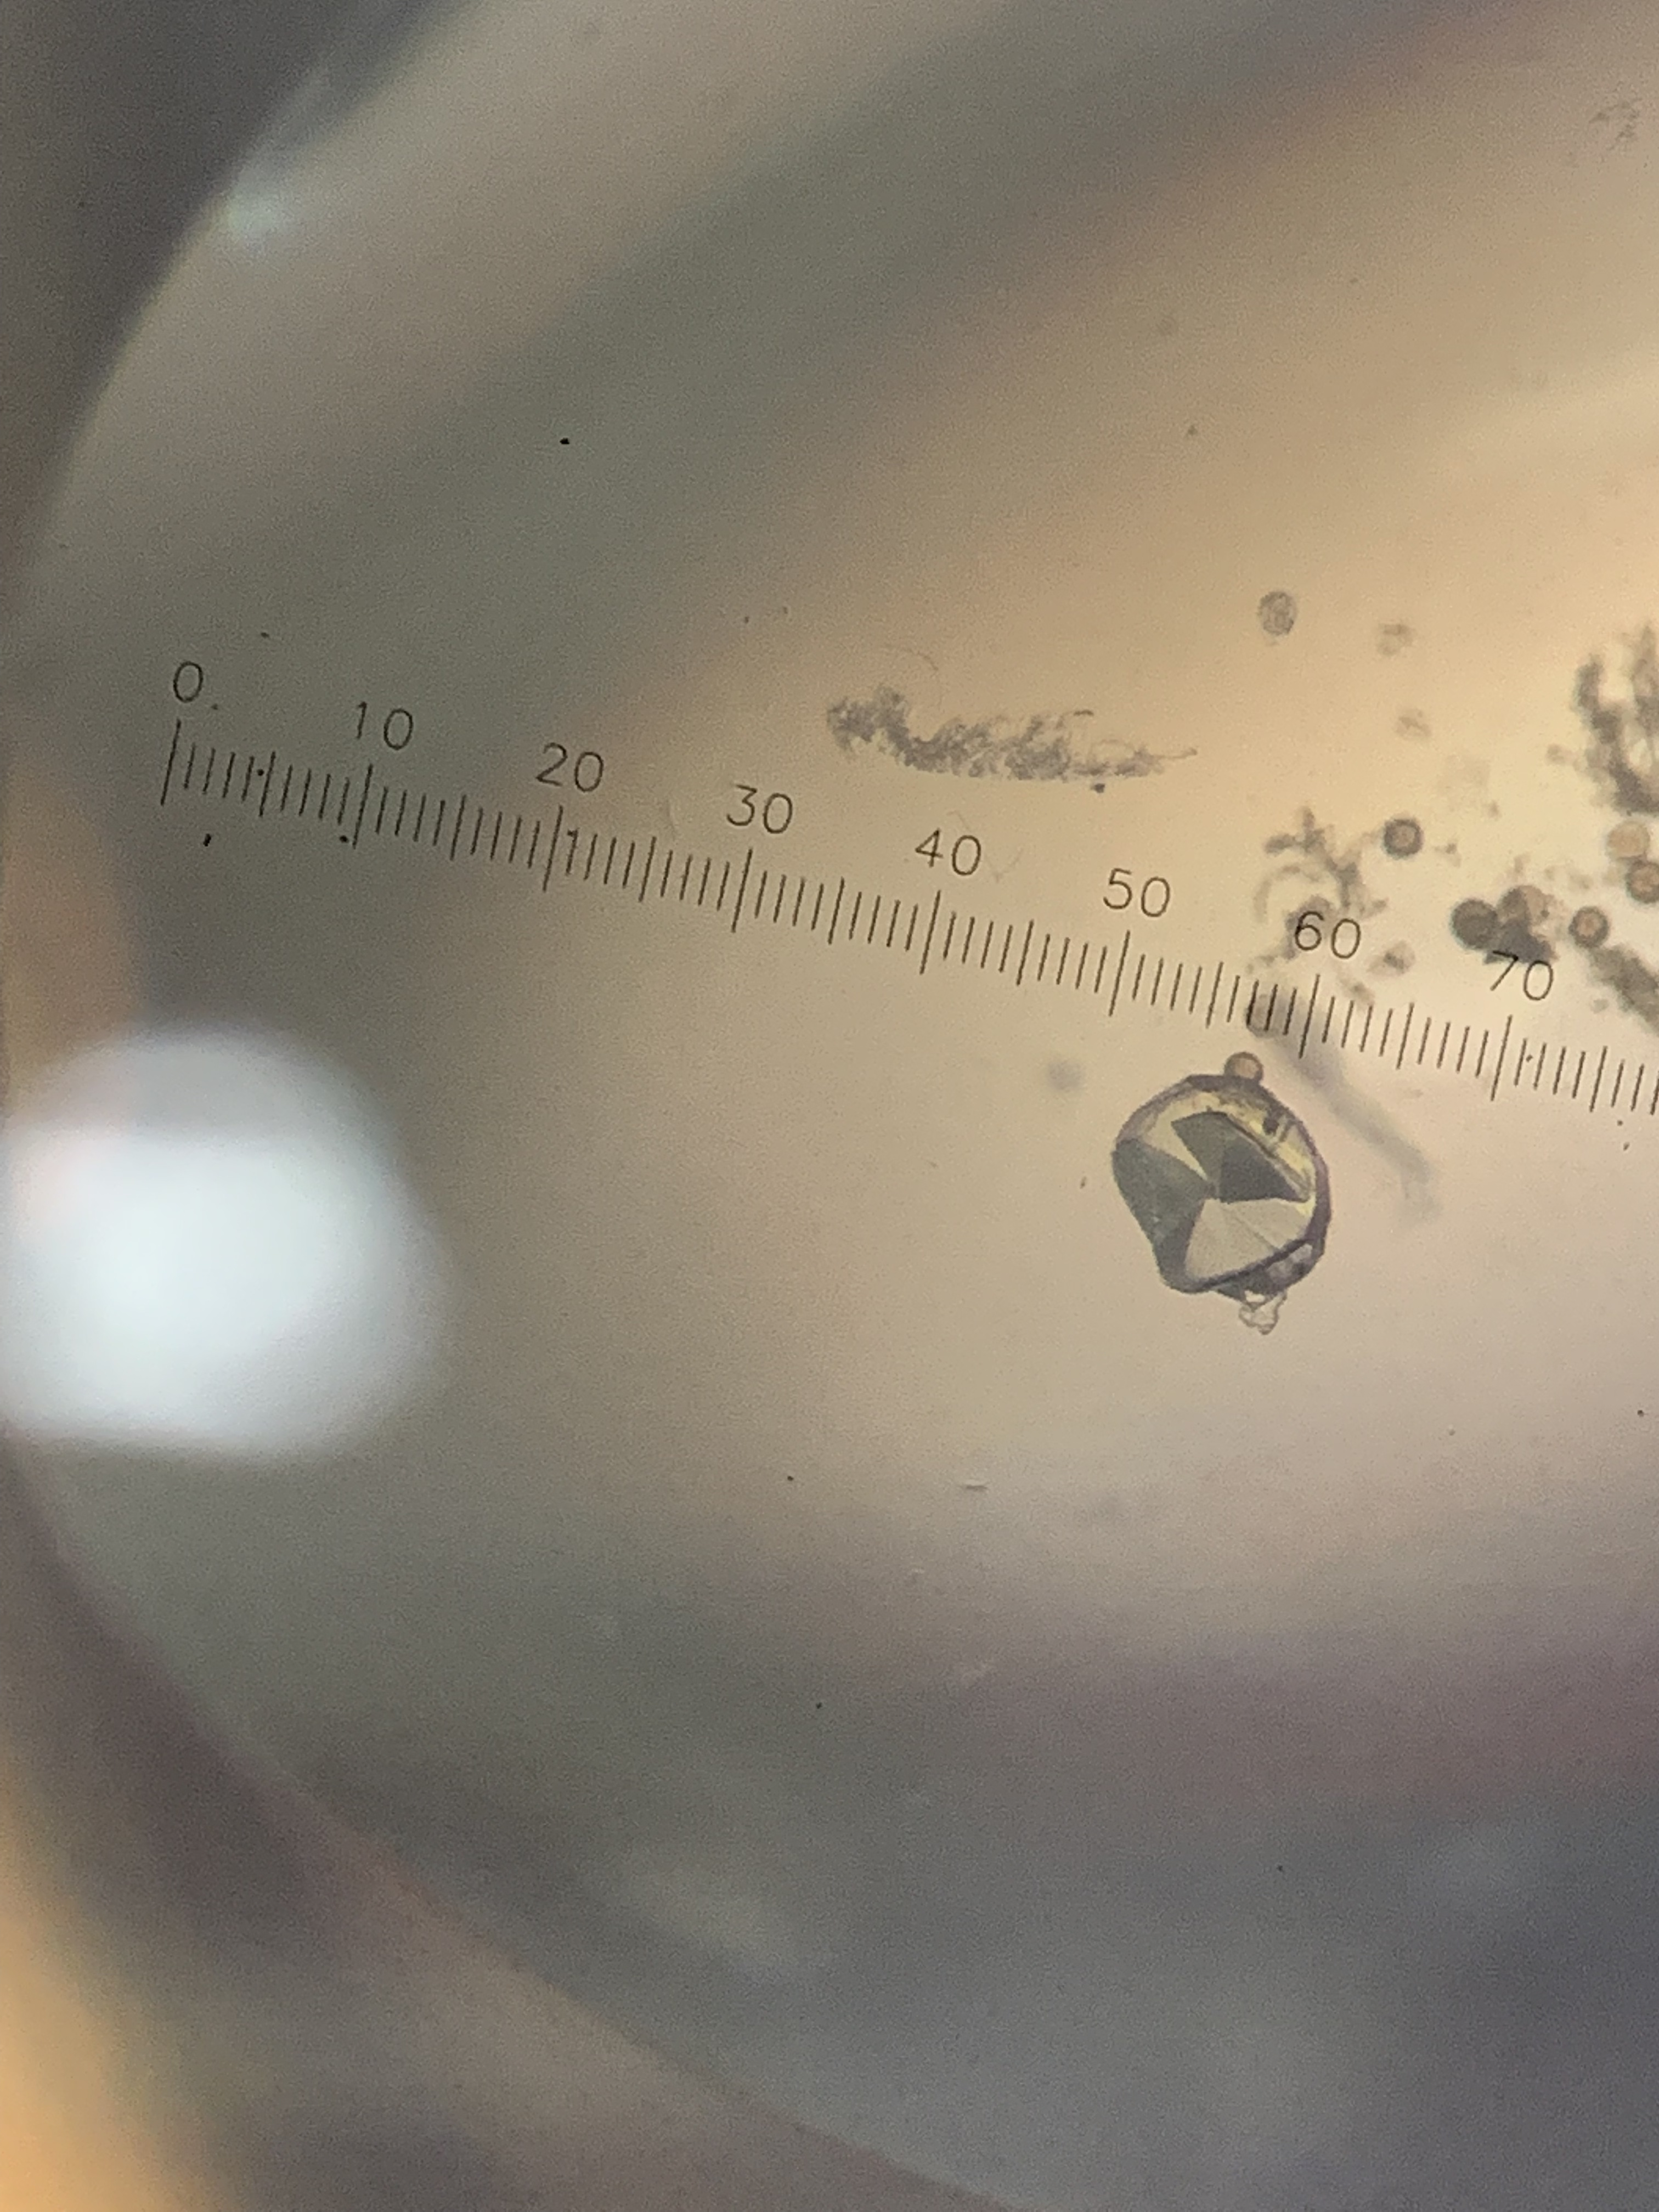
\includegraphics[clip, height=4cm]{imgs/se-1.jpg}
\hspace{1.6cm} 精製-1
\end{center}
\end{minipage}

\end{tabular}
\end{center}
\end{figure}


また、結晶のでき方の場合についてだが、沈殿剤の濃度が濃すぎると沈殿が生じてシャワー状の小さな結晶になり、薄すぎると全く結晶化しないと考えられる。今回は沈殿剤の塩化ナトリウムが濃い方ほどシャワー状になる可能性が高く、薄い方ほど全く結晶化しない可能性が高くなると考えられる。

\

\begin{tcolorbox}[colback=white,colbacktitle=black,coltitle=white,title={2}]
ブラッグの式を用いて実験で得られた回折像から測定の分解能を求めよ。
\end{tcolorbox}

観測された点のうちもっとも外側にあるものは中心との距離が61 mmであった。結晶からフィルムまでは40 mmなので、これをもとに分解能を求める。

\[ 40 \times \tan 2\theta = 61 \]
\[ \theta = 0.5 \arctan \frac{61}{40} = 0.495199\]
今回用いたX線の波長が $\lambda = 1.5418$ であるから、
\[d= \frac{\lambda}{2 \times \sin \theta}\]
に代入して
\[d= \frac{1.5418}{2 \times \sin 0.495199} = 1.62224\]
したがって今回の実験のX線結晶構造解析は高分解能と言える。
$1.5\mathrm{\mathring{A}}$ 
ほどの高分解能であればタンパク質に含まれる原子がほぼ分離して見えると言われている。

\part*{コンピューターによる回折強度の解析とモデル構築}

\section*{実験操作}
モデル構築ソフト「COOT」を用いてリゾチームのアミノ酸鎖のモデル構築を行う。

\section*{課題}
メールにて提出済


\part*{実習の感想}
タンパク質を結晶化してX線結晶構造解析をしたり、
モデリングソフトを用いてタンパク質のアミノ酸配列を考えたりするなど、
高度な実習ができたのがよかったと思います。
SDS-PAGEの電気泳動でマーカーの動きを観察し実際にリゾチームが精製できていることを確かめられたことができたのはよかったですが、それまでの工程の内容が複雑で少ない説明の中理解しながら実験を進めるのが大変でした。

\end{document}